% Created 2023-05-19 Fri 16:20
\documentclass[9pt, b5paper]{article}
\usepackage{xeCJK}
\usepackage[T1]{fontenc}
\usepackage{bera}
\usepackage[scaled]{beraserif}
\usepackage[scaled]{berasans}
\usepackage[scaled]{beramono}
\usepackage[cache=false]{minted}
\usepackage{xltxtra}
\usepackage{graphicx}
\usepackage{xcolor}
\usepackage{multirow}
\usepackage{multicol}
\usepackage{float}
\usepackage{textcomp}
\usepackage{algorithm}
\usepackage{algorithmic}
\usepackage{latexsym}
\usepackage{natbib}
\usepackage{geometry}
\geometry{left=1.2cm,right=1.2cm,top=1.5cm,bottom=1.2cm}
\usepackage[xetex,colorlinks=true,CJKbookmarks=true,linkcolor=blue,urlcolor=blue,menucolor=blue]{hyperref}
\newminted{common-lisp}{fontsize=\footnotesize} 
\author{deepwaterooo}
\date{\today}
\title{ET 框架拖拉机项目试改装}
\hypersetup{
  pdfkeywords={},
  pdfsubject={},
  pdfcreator={Emacs 28.2 (Org mode 8.2.7c)}}
\begin{document}

\maketitle
\tableofcontents


\section{双副牌双升108 张卡牌游戏}
\label{sec-1}
\begin{itemize}
\item 【游戏可试玩程序】:放在Release/Tractor.exe. Windows 用户大家可以下载试玩儿体验一下。
\item 昨天晚上找见了别人几年前就开发出来的卡五星麻将,所以写麻将游戏的想法就被恶杀在摇篮中。现在再写什么好呢?就只能写【双升拖拉机】了,就是两副牌108 张来打的拖拉机。现已经 ios iPhone 上有的双升游戏,可能搜索一下设计,写安卓版的双升了,看下能否套用ET 框架,写成四人网络【客户端与服务器双热更新的】网络游戏
\item 现在先搜索必要的框架设计,出版规则比大小算法之类的。
\item 【服务器与客户端的同步】:尤其是在分四人牌后,亮主拖底的时候,谁先亮,亮什么主,顺序重要,结果重要。【 ET 框架有专用的游戏服,由游戏服来状态同步】在本程序中,采用的是服务器保存所有的状态,处理所有的逻辑。比如,客户端在点击亮主后,做的事情就是发一个消息给服务器,不做任何显示操作,等待服务器传来亮主的消息后再显示
\begin{itemize}
\item 【发牌,公正性】:随机分牌。第一步就是要发牌。需要做到一个完全随机的发牌,就要保证每张牌发到每个玩家手里的概率都是一样的,而且牌的顺序是等概率随机打乱的。程序中采用的是如下的发牌算法(感谢Dr.Light提供):假如有两幅牌,编号从1到108,首先随机选出一个,并且将牌发给玩家,然后将这个编号的牌与108号牌交换编号,那么剩下的牌就是从1到107号。于是再从中选出一个,重复以上的过程,这样一来,算法的复杂度就是O(n)。
\end{itemize}
\item 【牌的逻辑OOD/OOP】设计:三个类,对应单张,拖拉机(对子是长度为1 的拖拉机),和混合单张与拖拉机
\item 第一手牌与非第一手牌的处理:
\end{itemize}

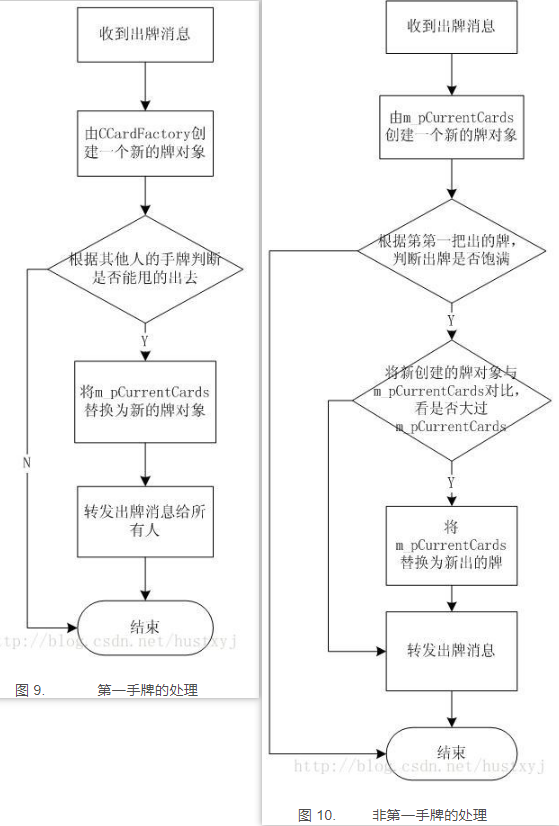
\includegraphics[width=.9\linewidth]{./pic/plan_20230508_223827.png}

\begin{itemize}
\item 参考一个很Q 的界面:
\end{itemize}

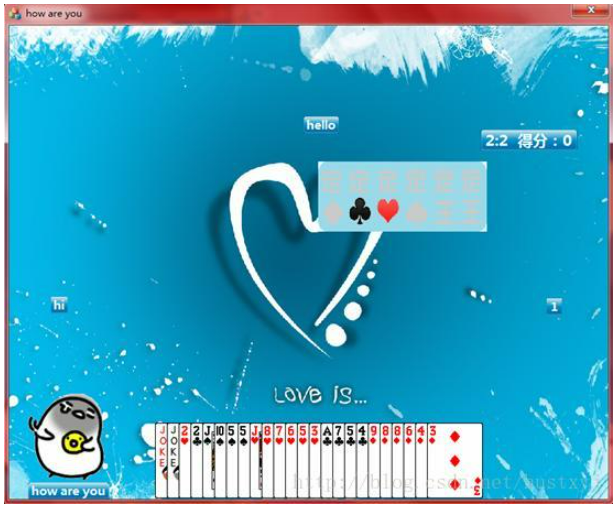
\includegraphics[width=.9\linewidth]{./pic/plan_20230508_222717.png}

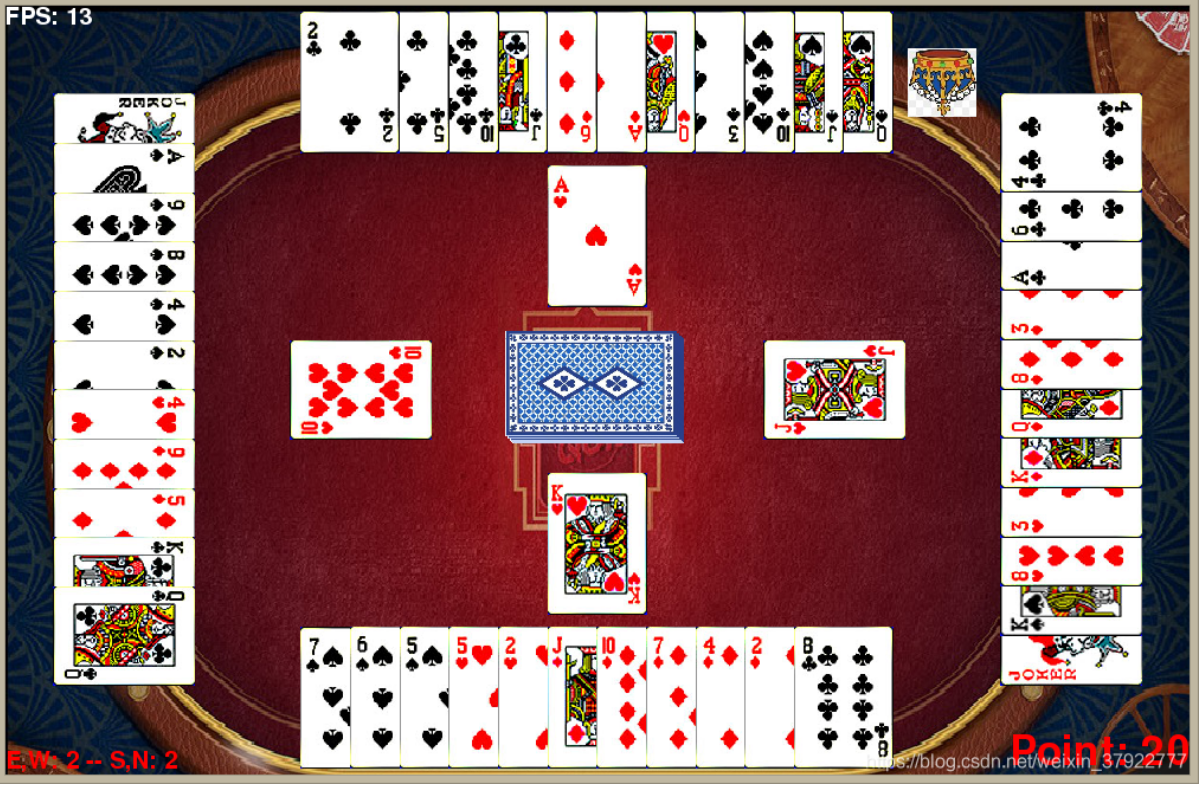
\includegraphics[width=.9\linewidth]{./pic/plan_20230508_221732.png}
\begin{itemize}
\item 亮着牌打的不好玩,一定会把其它三副牌藏起来的
\item \url{http://www.homygame.com/ngscom/help/shengji.htm}
\item 简易版设计原理:模拟拖拉机(升级)玩法;
\begin{itemize}
\item 1.创建两副牌的集合:HashMap
\item 2.创建纸牌:四个花色共108张♦ ♣ ♥ ♠
\item 3.创建poker的ArrayList操作集合
\item 4.创建亮主牌的操作
\item 5.将所有牌放入牌盒中
\item 6.创建四个玩家与底牌的集合:HashSet wj1,wj2,wj3,wj4,dipai
\item 7.洗牌
\item 8.发牌操作
\item 9.创建看牌方法
\item 10.调用方法看牌
\end{itemize}
\item 安桌上的游戏现在是这样的:还要再写一个吗?【活宝妹就是一定要嫁给亲爱的表哥!!!】还是说更为完善或是好玩儿的游戏逻辑?或是UI 视图画面,或是性能表现?反正一定是套用ET 框架写得最容易快速方便。【感觉现在这个截图的UI 长得有点儿丑怪。。】不好看不经典,看了就不想玩儿了。。
\begin{itemize}
\item 主要想要改进的地方:前辈十年前开发出的游戏,游戏整体【差强人意】现官宣的现项目基础上,主要游戏逻辑与改进方向【除了重构适配ET 框架以实现客户端服务器双端热更新, besides之外】如下。
\end{itemize}
\item \textbf{【界面设计:】} 八十年前没有ET 框架,不知道原作者是如何设计这个游戏的。感觉游戏的整体走桌面游戏风,要把菜单设计等改成【手游风格】。
\item \textbf{【逻辑设计,用户意愿:】} 不【尊重用户游戏配置选择】的游戏,永远是固执不受欢迎的。【游戏逻辑、玩法】需要能够给用户留足选择配置空间,如下:
\begin{itemize}
\item 现有的游戏规则:再找了理解一下:现找到原项目中提到这些。但作为程序员,不把它所有相关逻辑读懂,都感觉不明白它说的狠多是什么意思
\end{itemize}
\end{itemize}

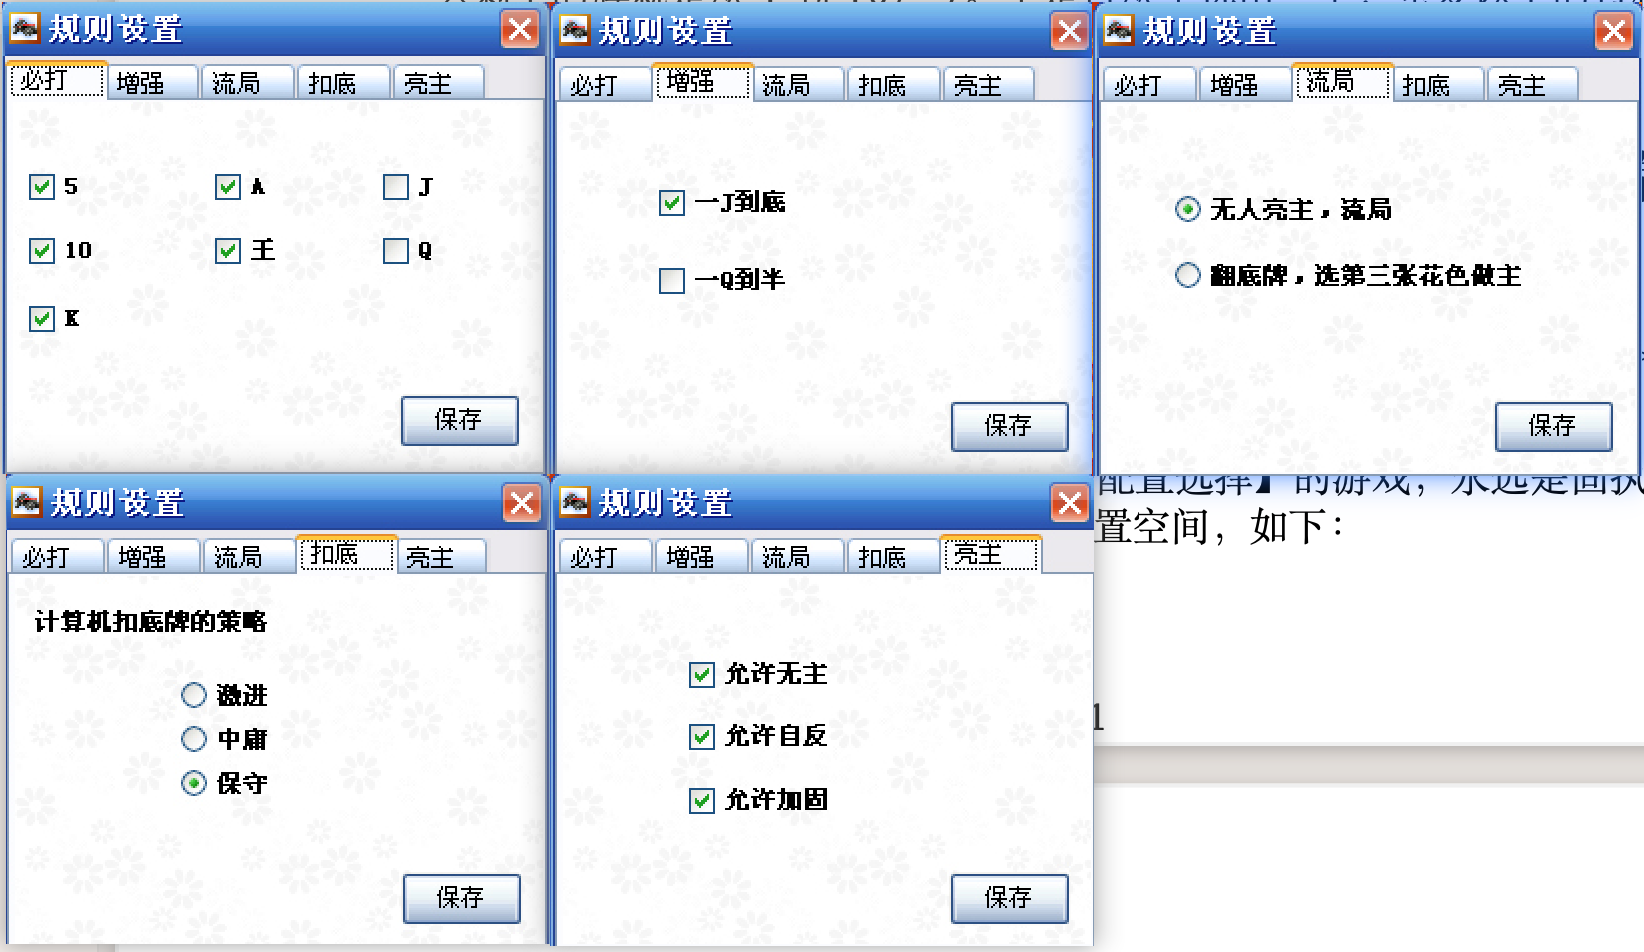
\includegraphics[width=.9\linewidth]{./pic/readme_20230510_160604.png}
\begin{center}
\begin{tabular}{ll}
\hline
配置用户选项 & 选项的功能说明\\
\hline
\textbf{2 为常主} & 是常主,就常主会比较多,尤其打王的时候;否则常主少,尤其打王的时候\\
\hline
\textbf{单 J 勾到6, 双 JJ 勾到 2} & 开历史倒车,增加游戏的无穷乐趣:惊险刺激:逢对家对J, 谁不想把对方废到6 或是2?\\
 & 逢自家打到J, 会想要被对方废到6 或是2?\\
\hline
\textbf{5 10 K 必打} & 因为比较难打\\
\textbf{逢 J 必打} & 因为上面不能言说的【惊险刺激】,不给任何双方逃跑的好玩机会\\
\textbf{J Q A必打} & 因为他们所添加的各种乐趣。若是J 与Q 合并为JJ, 则Q 可以跳过\\
\hline
\textbf{小光升1 级,大光连升3 级} & 不满 40 算小光,0 分为大光头。。。连升三级\\
\hline
游戏亮牌与反牌逻辑完善 & 添加闲家反牌时急速填扩张抠牌底分的机会\\
\hline
\textbf{捡分方扣底,底分翻倍} & 单扣乘2, 双扣乘 4, 甩牌或是拖拉机扣,则牌的张数,乘以 2.\\
 & 如此,才能让捡分方快速超越,以风马牛不能及之势火箭升级。。。\\
\hline
\end{tabular}
\end{center}
\begin{itemize}
\item \textbf{【关于J Q】}, 游戏设置: 
\begin{itemize}
\item 增强的规则:在一些地方流行一J到底、Q到半的玩法。
\item 庄家在打J时,如果下台,并且最后一把被J抠底,那么此庄家再上台时将从2开始打。
\item 庄家在打Q时,如果下台,并且最后一把被Q抠底,那么此庄家再上台时将从6开始打。
\end{itemize}
\item \textbf{【亮主规则】} :可以选择是否允许自反,加固和亮无主
\item \textbf{【亮牌规则】} :(注:以打8为例) \textbf{【这里有狠大的游戏逻辑改进,和游戏用户体验提升空间】}
\begin{itemize}
\item 在发牌过程中,第一次亮出的8的花色作为主牌花色。
\item 有以下几种情况可改变或加强主牌花色:
\begin{itemize}
\item 自保
\item 反主
\end{itemize}
\item 以上后三条以先出现者为准。
\item 若发牌结束仍无人亮牌,则以底牌第一张的花色作为主牌花色。
\end{itemize}
\item 以上三点应该是自己着重想要改进的地方
\item \textbf{【轮庄规则】} :为创造出好玩儿的玩法,这里是可以优化改进的。对家的本意是,两人合作,快速升级,所以需要两者配合。不需要,或可以配置不规定严格的顺序,给予他们无数无限合作可能,给予对方继续反副反主的机会,增加游戏趣味。
\begin{itemize}
\item 开局中,双方争庄,先亮者为庄家。
\item 庄家升级时,下一副牌由其对家当庄家。
\item 闲家上台时,下一副牌由此副牌的庄家的下家当庄家。
\end{itemize}
\item 其它这里没有列出来的,主要是我现在还不曾了解那些是在说什么,比如下面网络上提到过的:提供六种配置选项: \textbf{【允许自反】,允许对家保,允许反无将,A 必打} (是为什么呢,K 易跑光,不好捡分?)等
\item \textbf{【点击触屏、用户交互的性能优化】} :需要优化。玩家就算玩得不久,一直点鼠标,也是痛苦的事。需要AI 辅助,智能帮助用户出牌,让鼠标点击、选牌聪敏、反应快。
\begin{itemize}
\item 原游戏应该是桌面游戏,所以会有快捷键设置。但手游,就需要自己将触屏设置优化出来
\item 【去想】:怎么才能既有良好的用户触屏点击的反应灵敏性,又不失传统方式紧密摆牌?因为不同于桌面游戏,鼠标可以精准点击到位,手游上手指触屏的射线检测,视图上摆放过于紧密可能不利用射线检测成功,点击灵敏度降低。需要好好考虑一下手游上如何实现优化。这处牌又比麻将窄了狠多,确实不好检测。
\end{itemize}
\item \textbf{【逻辑设计,用户意愿:】}: 逻辑上,为能实现以上种种好玩玩法,游戏逻辑需要 \textbf{规定,约束严格的反牌规则:从高到低为【王黑红梅方】} ,就是别人叫方块的主,其它都可以反,但若是已经反到黑桃,接下来就只能反王或说是常主。允许捡分方按照以上规则反牌,这样才给给予捡分方底牌放 80 分,拖拉机扣底,火箭升级的机会。规则明确,公正。现游戏中一个【“流局”】界面,抹杀了这一切好玩儿的过程与结果,太不好玩了。。。游戏界面,也需要必要的文字提示等,帮助玩家理解游戏中的这些好玩儿规则,让玩家上瘾。。。
\end{itemize}

\section{主要参考项目:}
\label{sec-2}
\begin{itemize}
\item 【ET- 斗地主游戏】年代久远,ET 框架的版本古旧。手游风格的界面设计
\item 【ET- 卡五星游戏】年代久远,ET 框架的版本古旧。主要看牌类相关的房间内的逻辑
\item 分支 7.2 与主分支的区别:都有最开始必须取消主相机。区别是进入地图时,7.2 如果再激活相机,可以看见地图,小人也能跟随鼠标右键动。主分支可能还需要我再看一下,为什么主分支进入不了地图。两个分支对比一下,主要是让自己放心,现所使用的主分支应该没有 blocking 【BUG:】存在。去看下主分支,可以显示地图吗
\item 消息,没再区分热更新的消息,分成了内网与外网消息
\item 截几个斗地主游戏里的流程图供自己写时参考:
\end{itemize}

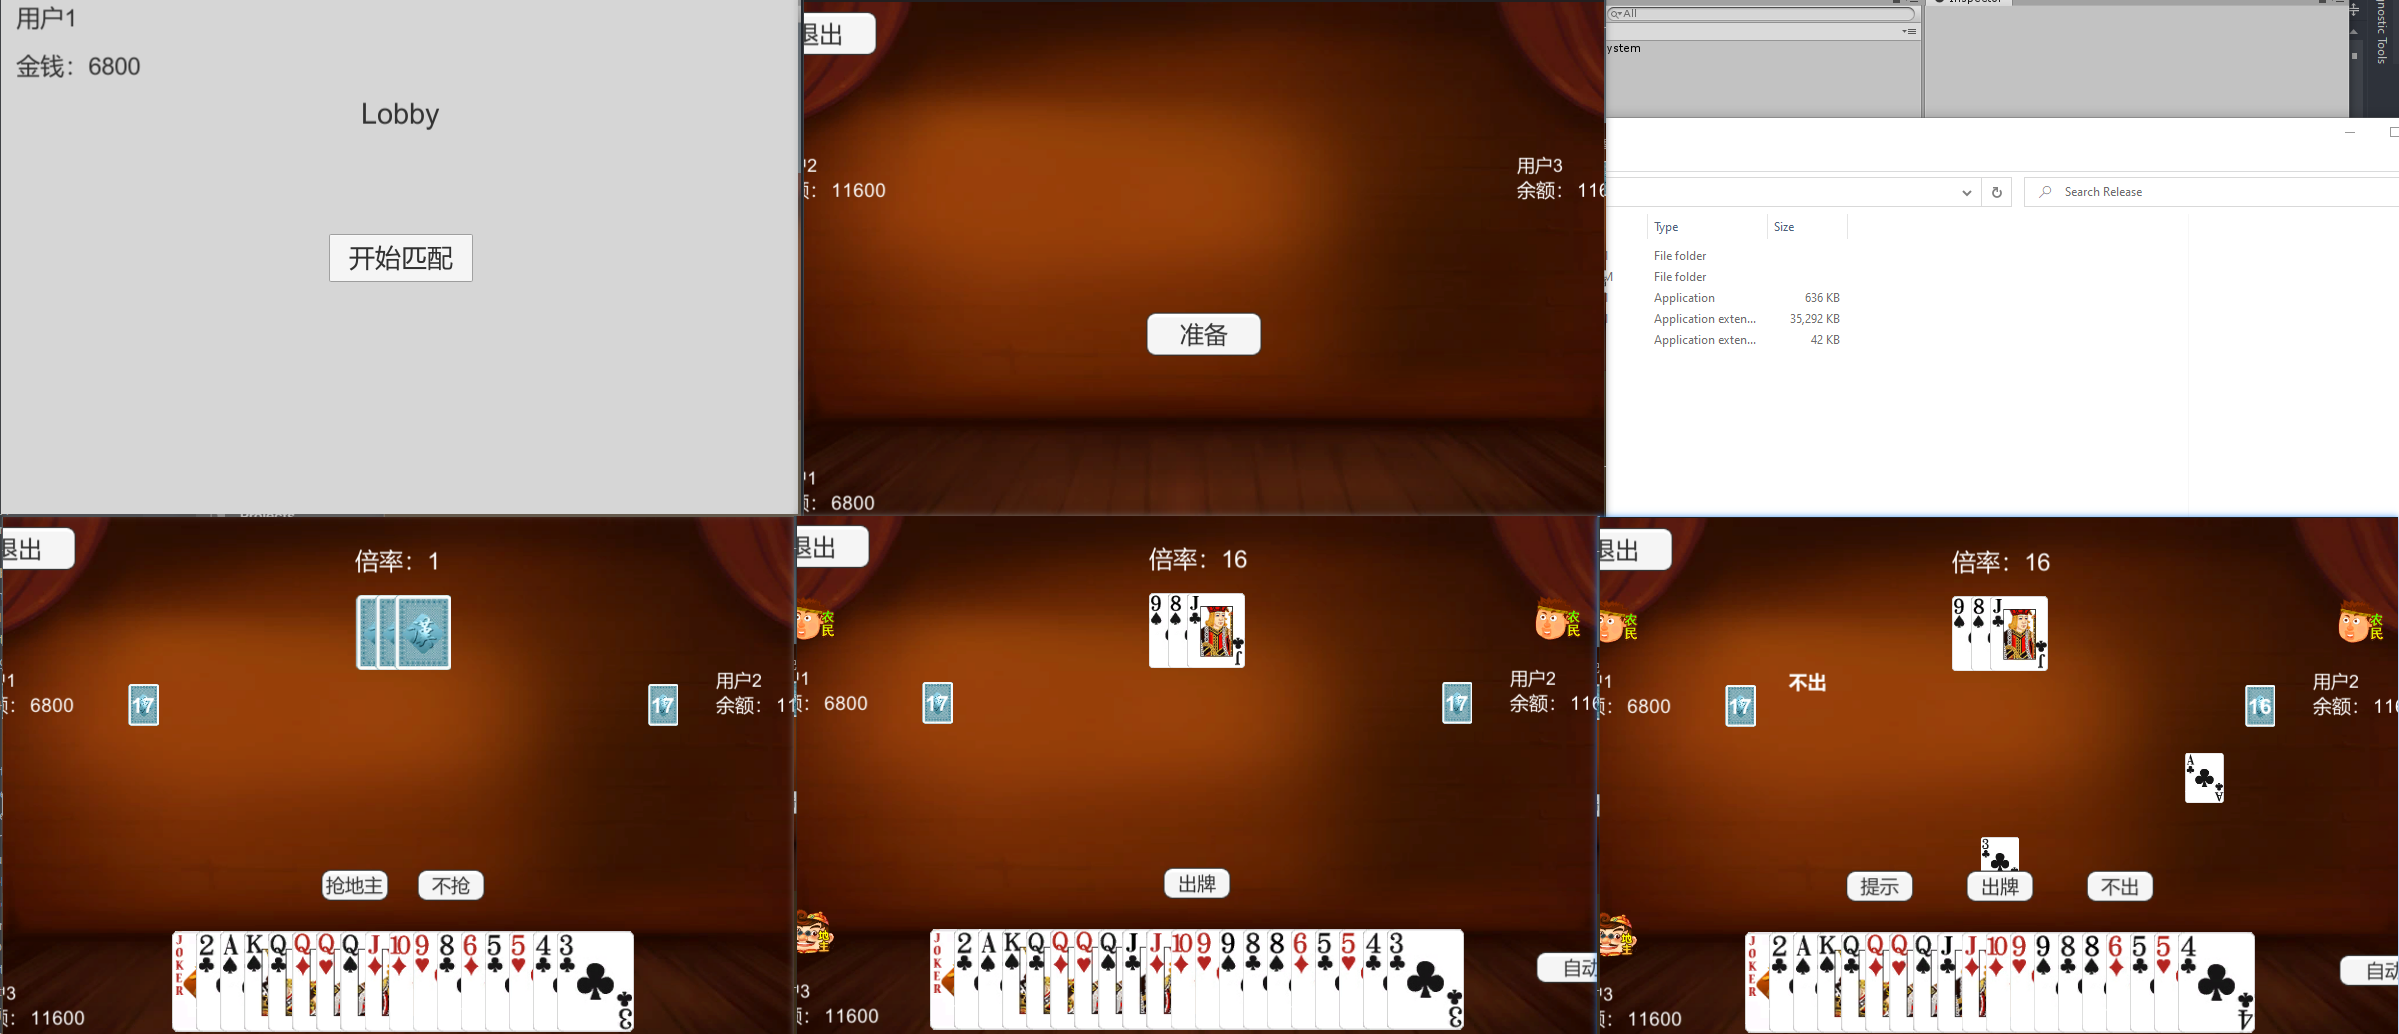
\includegraphics[width=.9\linewidth]{./pic/readme_20230511_163501.png}
\section{项目主要进展}
\label{sec-3}
\begin{itemize}
\item 因为两个参考项目的版本都狠古旧,现用最新版本的ET 【我觉得这里,最好我还是先去试ET7.2 官方版本可能更好】就以自己能有的相对快速,按照现有的理解,把能重组的重组出来。不理解的,再去看下两个项目分别的实现逻辑。
\item UILobby 的三个命令按钮狠好创建,但因为接下来的逻辑没能创建连通,程序仍然是运行不通,出报错。接下来应该是一段时间程序都极可能报错。但会试着修改每个界面上的错,把这个游戏的重构任务完成。
\item 现在的游戏主要是参考斗地主游戏,并根据最新ET7 框架的重构来,来重构自己的游戏,会在现各种文件报错的基础上一一修改掉所有的错,直到自己的游戏重构结束。因为对自己有绝对的自信,相信自己,就不怕它会出现的各种报错。真正改起来,也是 a-piece-of-cake 一口咬下。。。拿下。。。【爱表哥,爱生活!!!活宝妹就是一定要嫁给亲爱的表哥!!!】
\item 程序本身感觉不到困难,会试着解决过程中遇到的所有问题。只是今天状态不够,晚上会给妈打电话,会试着建几个 Unity 上会要用到的预设,再不行,今天晚上就早点儿休息。【任何时候,活宝妹就是一定要嫁给亲爱的表哥!!!】
\item 感觉程序的逻辑现在已经比较简单了:但是仍然需要花点儿时间,来熟悉这个重构过的ET 7 框架。今天下午会熟悉一部分,剩余未完成的明天上午来完成。今天熟悉划重点,与自己游戏的重构相关的重点。比如 \textbf{先前的多服务器系统变成为现在的服务器的路由系统,}, 不同层级的路由?网络调用下的各种Helper 类,比如 LoginHelper, 其它 Helper 等
\end{itemize}
\section{残余的几个小 bug}
\label{sec-4}
\begin{itemize}
\item 当进入UILobby 的时候,要把前面的 UILogin 删除。应该是有逻辑,只是因为我现在的【BUG:】,后面就座地执行的逻辑中断了
\end{itemize}
% Emacs 28.2 (Org mode 8.2.7c)
\end{document}